\documentclass[14 pt]{extreport}

\usepackage{extsizes}
\usepackage[utf8]{inputenc} %pour accents
\usepackage[T1]{fontenc}	%pour accents
\usepackage[francais]{babel}%pour langue
%\usepackage[textwidth=18cm,textheight=22cm]{geometry} %mise en page
\usepackage{hyperref}	%URL
\usepackage{listings}	%code
\usepackage{amsmath}
\usepackage{graphicx}
\usepackage{epstopdf}
\usepackage{lipsum}
\usepackage{smile_template}
\usepackage{fancyvrb}
\usepackage[section]{placeins}
\usepackage{float}% If comment this, figure moves to Page 2
\epstopdfsetup{outdir=./}

\usepackage{fancyhdr}


\pagestyle{fancy}
\setlength{\unitlength}{1mm}
\addtolength{\headheight}{1.5\baselineskip}
\renewcommand{\headrulewidth}{0.4pt}
\renewcommand{\footrulewidth}{0.4pt}
\rhead{
%
\includegraphics[width=3cm]{images/Logo_Smile_400.jpg}
}

% Redefine the plain page style
\fancypagestyle{plain}{%
  \fancyhf{}%
  \fancyfoot[C]{\thepage}%
  \renewcommand{\headrulewidth}{0pt}% Line at the header invisible
  \renewcommand{\footrulewidth}{0.4pt}% Line at the footer visible
}

\title{\textbf{Rapport de stage de fin d'études}}
\author{Martin Guilloux}


\begin{document}

\maketitle


\section*{Résumé}
Dans le cadre de ma dernière année d'études à l'INSA Centre-Val-de-Loire, j'ai effectué un stage de six mois, l'aboutissement de trois ans passés à l'institut. J'ai effectué ce stage au sein de l'équipe Outsourcing de l'entreprise Smile, à Montpellier. Smile est une entreprise d'hébergement et de développement de websites/webservices française, s'appuyant pour cela sur le monde de l'Open Source.

Ce stage m'a fait expérimenter plusieurs technologies, notamment liées à l'automatisation et à la virtualisation.

\section*{Remerciements}
Je remercie mon enseignant référent Benjamin NGUYEN, d'avoir encadré le déroulement de mon stage.\\
Merci également à Mathieu BLANC, mon maître de stage, pour sa bonne humeur et ses bons conseils. Et aussi pour les parties de Mario Kart ;)\\ % Même si à la fin c'est moi qui gagne
Je remercie aussi toute l'équipe Outsourcing de Smile Montpellier, pour l'accueil et la bonne ambiance quotidienne : Syben, Daber, Adbig, Cebri, Wibru, Secal, Jocor, Dyfei, Segir, Mohla, Aulem, Flmag, Pamar, Alniz, Niper, Alwie, merci d'avoir été plus que de simple collègues de travail.\\
Merci aussi à tout le reste de l'équipe Smile Outsourcing, avec qui j'ai discuté au quotidien. 


\tableofcontents

\newpage
\subsection*{Summary}

For the last six months I have been in a internship in Smile, a multinational (but mostly french) company that focuses on the development and hosting of websites. The main theme on this internship was the automation and industrialisation of deployment processes on new platforms hosted by Smile.

In order to achieve this goal I divided my work between upgrading current software architecture based on puppet, an orchestration and automation tool that runs on every node in the production system ; and adding another orchestration tool, Ansible, to the system.

At first the project was heading towards the complete elimination of puppet from our system, replacing it with Ansible. But as we explored Ansible we came to realisation that it could not replace Puppet entirely, though it could take off some load from the puppet master server. In the end we decided to integrate Ansible as a side tool to deploy new hosts and virtual machines, and to create a new puppet master server with the latest version of Puppet so that we could integrate specific projects using (for instance) Debian 9 or PHP 7.
\subsection*{Keywords}
Automation, DevOps, Hosting, Linux systems


\chapter*{Glossaire}

\begin{itemize}
\item{\textbf{Automatisation}}: Ensemble de techniques permettant le déroulement autonome d'un système, en interconnectant plusieurs élements de ce système ; Par exemple, la génération d'un fichier pdf et l'envoi de ce fichier par mail, tout ceci sans intervention directe humaine.

\item{\textbf{Container}}: système d'exploitation isolé à l'intérieur d'un autre système, permettant ainsi à un hôte de virtualisation de faire tourner plusieurs systèmes sur une seule machine physique. (ex. de systèmes de conteneurisation : docker, lxc, openVZ)

\item{\textbf{Orchestration}}: Processus automatique d'organisation, de coordination et de gestion de systèmes informatiques, de middlewares et de services.

\item{\textbf{Ansible}}: Plate-forme logicielle d'automatisation Open Source en python, détenue par Red Hat. Ansible s'appuie sur ssh et utilise un modèle agentless ne nécessitant pas d'installer un client sur chaque noeud géré.

\item{\textbf{Puppet}}: Une autre plate-forme logicielle d'automatisation Open Source, écrite en ruby, développée par Puppetlabs. Puppet est basé sur un modèle master-slaves, il est nécessaire d'installer un agent sur chaque noeud, qui exécute le catalogue d'instruction envoyé par le puppetmaster.

\item{\textbf{PXE}} (prononcé Pixie): Système permettant à un serveur de booter sur une image de système d'exploitation présente sur le réseau

\item{\textbf{ENC}}: Pour External Node Classifier - Programme externe à Puppet interrogé par le puppetmaster, chargé de gérer pour chaque noeud la liste des classes et des paramètres qui lui sont attribués. (Par exemple, l'outil puppet-dashboard, en plus de fournir une interface web de résumé des puppet run, offre aussi la possibilité d'être utilisé comme ENC)

\end{itemize}

\chapter{Introduction}

\section{Cadre et objectifs du stage}

\subsection{Le stage}L'intitulé de mon stage, "Industrialisation des méthodes de déploiement de plates-formes d'hébergement Internet", suggère la mise en place et la convergence de plusieurs outils pour améliorer à la fois les temps de traitement et la qualité des déploiements de plates-formes d'hébergement. Dans cette optique le travail a été décomposé en plusieurs phases, la première consistant à comprendre le fonctionnement du système existant, l'architecture réseau des serveurs de production de Smile, la base technique en place, ainsi que le périmètre impacté par l'ensemble des modifications à apporter. Il a fallu ensuite mettre en place ou améliorer des solutions dans un souci d'amélioration continue, tout en maintenant et en adaptant l'existant de manière à permettre la cohabitation entre les systèmes de production d'aujourd'hui et de demain.

Avant de parler plus en détail des tâches que j'ai été amené à accomplir, je vais rapidement faire une présentation de l'entreprise qui m'a accueilli pendant ces six mois.

\subsection{Présentation de Smile}

\subsubsection{Présentation générale}
Smile est une société fondée en 1991\footnote{qui est aussi l'année du lancement du World Wide Web et de la mort de Freddy Mercury. Comme quoi.}, par Alain Arditi, Patrice Bertrand, Cyrille Chignardet et Jérôme Prompsy. La société se place à ses débuts sur le secteur des applications clients/serveur développés en mode RAD.

En 1995-6, Smile profite de la démocratisation du World Wide Web et met en place le premier site bancaire sur le web pour le compte du Crédit Lyonnais.En 2001 Smile amorce un virage et entre dans le monde de l'Open Source et continue de croître jusqu'à présente dans de multiples bureaux en France, en Espagne, en Belgique, au Luxembourg, en Suisse, au Pays-Bas, en Ukraine, en Côte-d'Ivoire et au Maroc.

A l'heure actuelle, Smile compte environ 1200 employés répartis dans dix-huit agences, et continue de développer son coeur de commerce sur les technologies du web (Développement web, CMS, e-commerce, décisionnaire, Cloud computing, hébergement...) mais aussi depuis peu dans l'IoT, et ce toujours en se basant sur des technologies et des logiciels Open Source.

\subsubsection{Présentation de l'équipe Outsourcing}

J'ai effectué mon stage dans l'équipe Outsourcing de Smile, en charge du réseau de production de Smile et de l'hébergement des sites web et des webservices. Cette équipe est répartie entre l'agence de Paris et l'agence de Montpellier (où j'ai effectué mon stage).

On distingue trois équipes dans l'entité \emph{Smile Outsourcing} :
\begin{itemize}
	\item Les chefs de projet (CP), en charge du déploiement de plateforme techniques et du suivi des projets techniques ainsi que des ressources associées selon les besoins exprimés par le client.
	\item L'équipe de production, dédiée au troubleshooting du système de production et aux demandes des clients concernant l'hébergement, ainsi qu'au traitement des tickets relevant également de ce périmètre
	\item L'équipe Infra, que j'ai intégré pendant la durée de mon stage, dont le périmètre est plus centré sur la maintenance et l'amélioration des outils internes, du réseau de production, ainsi que des serveurs physiques, sans contact direct avec le client.
\end{itemize}

\chapter{Découverte du réseau de production et de la base technique}

A mon arrivée chez Smile, j'ai commencé par effectuer un tour des technologies utilisées, ainsi que du réseau de production sur lequel j'allais être appelé à travailler. J'ai ainsi pu dégager les points sur lesquels il faudrait agir et isoler les problématiques des différents composants du système de production.

En parallèle je me suis documenté sur les technologies et les outils que j'allais utiliser tout au long de mon stage, notamment Puppet et Ansible.

\section{Présentation du réseau de production}

Les serveurs de production de Smile sont répartis sur trois \emph{datacenters} : Deux dans les environs de Paris (Equinix PA3 à Saint-Denis et Iliad à Vitry-sur-Seine), et un à Lyon (Datacenter SFR à Venissieux) rajouté récemment suite au rachat par Smile de OpenWide Outsourcing (OWO). La convergence avec OWO étant en cours, j'ai été amené à travailler uniquement sur des serveurs présent dans les DC de Paris. Dans chacun de ces deux DC se trouve un Core Router Cisco (cr1 et cr2) ainsi que deux firewalls (fw3,4 et fw5,6), à savoir des serveurs dell sous openBSD. Cette répartition entre plusieurs DC fait suite à la volonté de Smile de mettre en place un Plan de Reprise d'Activité (PRA) incluant des \emph{datacenters} distants de plus de trente kilomètres.

Les core routers et les firewalls sont interconnectés entre les deux sites par fibre optique et administrés sur un vlan spécifique, de même que les serveurs derrière les firewalls (sur un autre vlan).

\begin{figure}[htp]
\centering
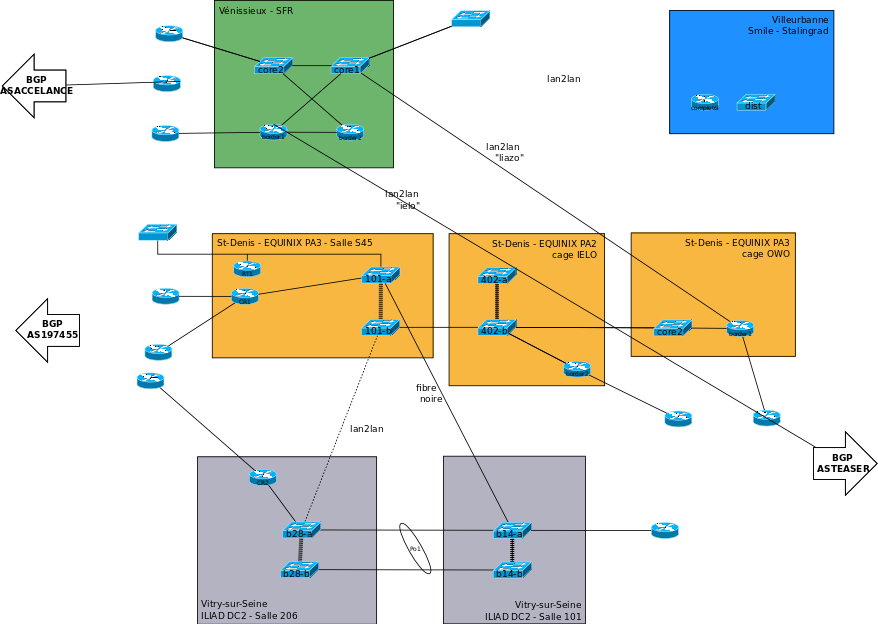
\includegraphics[scale=0.4]{reseau_backbone.png}
\caption{Schéma récapitulatif du réseau backbone de Smile}
\label{}
\end{figure}
%TODO insérer schéma réseau Smile
\section{Le socle technique de la production}

Je vais ici présenter un résumé des technologies utilisées par le système de production chez Smile, en deux parties : les technologies de virtualisation et le système de monitoring, et enfin le système d'orchestration en place, utilisant puppet dont je présenterai rapidement le fonctionnement.
\subsection{Technologies de virtualisation et de monitoring}
\paragraph{Virtualisation :}Les sites hébergés par Smile le sont dans des containers openVZ, avec pour hôtes de virtualisation des serveurs physiques tournant sous CentOS. Les VM sont nommées en fonction du client et du rôle qu'elles jouent dans le système du site web (par exemple youboost-postgresdb1.priv.smile-hosting.fr pour une VM de base de donnée de youboost, ou gifi-pp.priv.smile-hosting.fr pour une VM de pré-production). Les hôtes de virtualisation quand à eux sont nommés en fonction du client dans le cas d'un serveur dédié (ex. gifi-host3.vpn.ti.smile.fr) ou shared-host dans le cas de serveur mutualisé (les serveurs mutualisés sont cependant appelés à migrer vers un cluster utilisant KVM).

Le déploiement de nouveaux hôtes de virtualisation se faisait en PXE, puis sa configuration se faisait à la main ou par le biais de scripts shell.

%TODO schéma openVZ

\paragraph{Monitoring :}Le système de production possède plusieurs facettes qui nécessitent d'être monitorées : Il faut surveiller le bon fonctionnement des backups (basés sur bacula et des scripts utilisant rsync), mais aussi la charge réseau entre les différents datacenters (et potentiellement répartir la charge entre les deux DC), et enfin l'état de tous les serveurs de production.

Pour cela plusieurs outils sont utilisés : Pour les backups un outil interne remonte les informations sur l'état des backups via une page web, tandis que la charge réseau est surveillée via snmp et graphée avec \emph{Cacti}. Pour monitorer l'état des serveurs, enfin, Smile utilise un fork de \emph{Nagios} écrit en python : \emph{Shinken} ainsi qu'une interface web pour afficher ses données, \emph{Thruk}. L'équipe de production utilise également un outil interne de monitoring, \emph{suri5} pour monitorer les sites clients et pour remonter des alertes. Tous ces logiciels sont bien sûr Open Source (un mouvement fortement ancré dans le fonctionnement de Smile, même si cette tendance semble évoluer ces derniers temps).

\subsection{Présentation du système d'orchestration}

Le système d'orchestration à mon arrivée était entièrement basé sur Puppet, un système d'automatisation et d'orchestration Open Source édité par Puppetlabs et écrit en Ruby que je vais rapidement présenter.

Puppet est basé sur un système \textbf{agent-serveur}, c'est à dire que sur chaque noeud géré par puppet il faut installer un \textbf{agent} puppet (présent dans le paquet puppet de base) et le configurer pour se connecter au puppetmaster, le serveur gérant chaque noeud. Un service lance l'agent toutes les heures en temps normal, mais sur une architecture telle que celle de Smile, les temps de traitement excèdent cette durée, c'est donc un \emph{cron} qui lance une \emph{puppet run} deux fois par jour pour éviter la surcharge du puppetmaster (cette cron est générée elle-même lors de chaque run puppet, comme je l'expliquerai un peu plus loin)

Lors de cette run, l'agent se connecte au puppetmaster de manière sécurisée (la suite puppet inclut une autorité de certification qui permet d'ouvrir des connexions sécurisées par SSL). Une fois cette étape d'authentification effectuée, l'agent rassemble des informations sur le système sur lequel il s'exécute. Il envoie ensuite ces informations au puppetmaster, qui s'en sert pour génerer une série d'instructions qui sont renvoyées à l'agent, ce dernier les exécutant et renvoyant en fin de run un résumé de l'état de sortie de chaque instructions, permettant de constater les erreurs de traitement ou les fichiers modifiés (par exemple).

Ci-après, un schéma récapitulatif des interractions au cours d'une puppetrun. On peut constater que la run a lieu en trois temps, d'abord une connexion agent $\rightarrow$ master, pendant laquelle le noeud envoie ses informations (des \emph{facts}), puis master $\rightarrow$ agent, durant laquelle le puppetmaster envoie le catalog au noeud, et enfin une dernière connexion agent $\rightarrow$ master pour le reporting.

\begin{figure}[H]
\centering
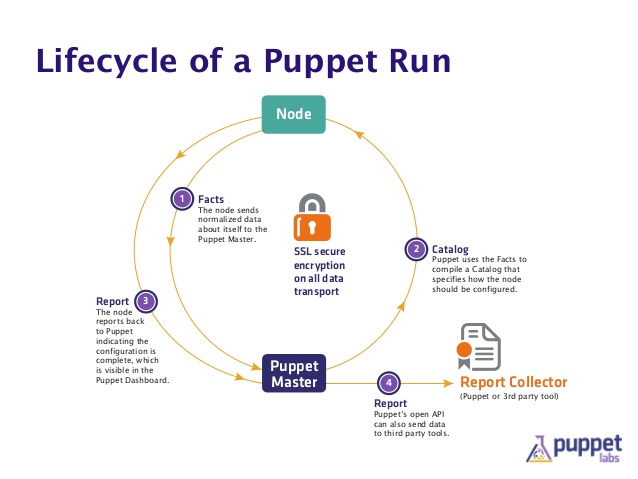
\includegraphics[scale=0.70]{puppetrun.jpg}
\caption{schéma volé éhontément dans une keynote puppetlabs}
\label{}
\end{figure}

Avant de poursuivre, il est nécessaire d'introduire un peu de vocabulaire spécifique à puppet.

Pour savoir quelles instructions exécuter sur un noeud, puppet utilise un système de \emph{manifests} écrits en "langage puppet", un langage à la syntaxe assez spécifique (voir un exemple de manifest puppet en annexe A) mais relativement simple à comprendre, ainsi qu'un système de \emph{templating} basé sur \emph{erb} (Embedded RuBy) pour pousser des fichiers de configuration sur les noeuds. Ces manifests se divisent en classes, elles-mêmes divisées en ressources. Avec puppet, tout est ressource.\footnote{Paracelse ajouterait que "rien n'est ressource, c'est la dose qui fait la ressource."} Une ressource est en effet l'unité fondamentale d'instruction en puppet. Par exemple, déclarer une ressource de type \emph{file} dans un manifest donnera l'instruction de transférer un fichier (depuis le puppetmaster ou n'importe quelle URI, ou encore d'après un template), tandis qu'une ressource \emph{exec} permettra d'exécuter une commande directement dans le shell de la machine distante (encore une fois, voir en annexe A pour un exemple de code puppet)

Par ailleurs, Puppet utilise un système dit de \emph{ressources exportées} pour partager des informations entre différents noeuds. Le principe est simple : En préfixant une ressource d'un arobase dans le code puppet, cette ressource est dite \emph{exportée}, c'est à dire qu'elle est stockée sur le puppetmaster dans une base de données appelée la puppetdb, et identifiée par un ou plusieurs tags.

Un type de ressource spéciale, appelé \emph{collector}, peut récupérer ces ressources par tag et les exécuter. Un exemple d'utilisation est de générer un fichier de configuration à l'aide des facts d'un noeud, mais de stocker le fichier ainsi généré dans la puppetdb, puis de le collecter sur un serveur qui a besoin de ce fichier de configuration (par exemple shinken)

\begin{itemize}
	\item Une classe est une suite de déclarations de ressources, qui peut être incluse dans un manifest (et ainsi éviter de retaper le même code plusieurs fois) avec des paramètres spécifiés lors de l'écriture de la classe. Par exemple une classe xmpp::client pourrait recevoir un paramètre pour savoir à quel serveur xmpp le client doit se connecter, afin de gérer les fichiers de configuration xmpp correctement.
	\item Un manifest, quant à lui, est un ensemble de ressources et d'inclusions de classes, en somme un fichier puppet générique.
	\item Un module Puppet est un ensemble de manifests, de fichiers, de répertoires et de templates rassemblés dans un but de portabilité. Il peut aussi contenir des fichiers ruby exécutés sur l'hôte distant pour générer des \emph{facts} supplémentaires.
	\item Un catalog Puppet est un ensemble d'instructions envoyées par le puppetmaster à un noeud après les avoir "compilées".
\end{itemize}

Ci-dessous, l'arborescence typique d'un module puppet.

\begin{Verbatim}[fontsize=\scriptsize]
magui@puppetmaster-v4:~/puppet/modules/puppetnode (bacula-lxc)$ tree
.
+-- files
|   +-- etc
|   |   +-- profile-lenny.default
|   |   \-- profile-lenny.puppet
|   +-- etc-default-puppet
|   +-- nrpe
|   |   \-- check_puppet.sh
|   +-- puppet.conf.preprod
|   +-- puppet.conf.prod
|   +-- puppet-cron-cleaning-tasks
|   +-- puppetlabs-pinning
|   \-- tools
|       \-- facter
|           \-- util-ip-patched.rb
+-- lib
|   \-- facter
|       +-- all_vzchildren_fqdn.rb
|       +-- interfaces_with_link.rb
|       +-- lamp_stack_versions.rb
|       +-- majdistrelease.rb
|       +-- pam_bash_users.rb
|       +-- puppetrun_cronjob.rb
|       +-- resolv_domain.rb
|       \-- utc_offset_hours.rb
+-- manifests
|   +-- announce
|   |   \-- register.pp
|   +-- announce.pp
|   +-- collector.pp
|   +-- config.pp
|   +-- cron.pp
|   +-- init.pp
|   +-- nrpe.pp
|   +-- puppetscript.pp
|   +-- service.pp
|   \-- tools
|       +-- all.pp
|       +-- facter.pp
|       +-- lsbrelease.pp
|       +-- puppetlabs_repository.pp
|       \-- ruby.pp
+-- metadata.json
\-- templates
    +-- collector-cron.part.erb
    +-- cron-smile-puppet.erb
    \-- puppet.conf.erb

\end{Verbatim}

\newpage
Une autre composante essentielle du système d'orchestration de Smile est l'utilisation de \emph{hiera}. Il s'agit d'un système permettant de stocker des variables en dehors des manifests dans des fichiers yaml. Dans le cas de Smile hiera est utilisé pour stocker les variables spécifiques à chaque serveur, permettant de gérer les spécificités de chaque machine de manière centralisée.

Lors d'une run puppet, le puppet-dashboard de Smile fait office d'ENC\footnote{voir le glossaire} pour déterminer quelles classes appliquer à chaque noeud. Il lit ensuite les manifests et les hieradata et les adapte au noeud en renseignant les variables (on pourrait faire une analogie avec l'étape des directives de préprocesseur dans une compilation), avant d'envoyer un \emph{catalog} au noeud qui les exécute.

Au cours de cette exécution puppet remplit des fichiers de configuration, installe des paquets à des versions spécifiques, transfère des fichiers de scripts, lance des services... A la fin d'une run puppet, on a donc un système dans un état donné, et refaire une run sans modifier de paramètre garde le serveur dans cet état (ou l'y remet si des fichiers ont été modifiés à la main). Cette idempotence est l'un des points majeurs sur lesquels puppet insiste : Il garantit une infrastructure dans un état stable, exempte de modifications à la main, et apporte donc des certitudes quant à l'état des configurations de chaque système.

\chapter{Les évolutions apportées}

Lors de mon arrivée chez Smile, l'équipe Infra, que j'ai intégré, était en pleine restructuration du fonctionnement interne. Nous avons ainsi mené plusieurs projets en parallèle que je vais présenter ici, notamment la mise en place d'un serveur puppetmaster en version 4 et la migration des modules puppet utilisés par smile, jusque là en version 2 ou 3 ; L'intégration de l'outil d'automatisation \emph{Ansible} au système d'orchestration de la production ; Et une étude pour déterminer le nouveau socle de virtualisation de Smile. En plus de ces tâches majeures, j'ai mené des missions parallèles s'apparentant plus à l'exploitation courante (optimisation/écriture de scripts, ticketing, fixs divers sur des manifests puppet...) que je ne détaillerai pas ici.

\section{Choix du socle de virtualisation}

Jusqu'ici, le socle de virtualisation utilisé par Smile était, comme décrit plus haut, une base CentOS comme système d'exploitation, et la suite OpenVZ pour déployer des containers. Cependant, le projet OpenVZ apporte son lot de contraintes : il nécessite un kernel spécial (vzkernel) sur l'hôte de virtualisation, et son développement s'est considérablement ralenti ces dernières années. Il a donc fallu réfléchir à la mise en place d'un autre socle de virtualisation avec plus de dynamique dans son développement, et idéalement plus d'avantages que son prédécesseur.

L'utilisation de containers plutôt que de machines virtuelles type KVM/QEMU s'est imposée pour des raisons de performances : L'écart de performances entre un container et un OS "bare-metal" est de l'ordre de 2 à 3\%, contre 5-6\% environ pour une machine type KVM. En termes de densité, il est possible de peupler un serveur avec 14 fois plus de containers que de KVM.

Notre choix s'est porté sur l'utilisation de LinuX Containers (\emph{lxc}), avec son \emph{daemon} lxd. Ce système de conteneurisation a depuis quelques années le vent en poupe, bénéficiant d'une intégration privilégiée au noyau Linux, dont il tire profit avec des features comme les cgroups et les espaces de nommages, qui permettent d'apporter une couche supplémentaire de sécurité aux containers. 

Cependant lxd, étant un produit de Canonical, n'est disponible que sous Ubuntu. C'est pourquoi il a été arrêté que les nouveaux hôtes de virtualisation de Smile sont maintenant sous Ubuntu Server 16.04, l'édition Long Term Support de Ubuntu Server.

\section{Intégration d'Ansible}

Un autre projet dans le cadre de l'amélioration et l'industrialisation de la production, nous avons intégré l'utilisation d'Ansible à l'ensemble des outils de Smile, que je vais brièvement présenter ici.

Dans un premier temps, le projet était de remplacer entièrement Puppet avec Ansible, mais au fur et à mesure de notre exploration de l'outil, celui-ci ne suffirait pas à combler les besoins que couvre Puppet. Il a donc été décidé de conserver Puppet tout en intégrant Ansible aux outils de Smile, pour toutes les tâches de déploiement afin d'alléger la charge du serveur Puppet.


\subsection{Présentation d'Ansible}

\subsubsection{Présentation générale}
Ansible est un "outil d'automatisation simple"\footnote{Du moins d'après ses concepteurs : \url{https://www.ansible.com/}}, fonctionnant sans agent au contraire de Puppet. Pour les noeuds à administrer, il suffit d'avoir un daemon ssh ainsi que l'interpréteur python installé. 

Ansible utilise ensuite une série de connexions ssh pour pousser des scripts python qui s'exécuteront sur le noeud. On a donc une architecture beaucoup plus simple que celle de Puppet puisqu'il suffit d'installer Ansible sur son poste pour pouvoir gérer immédiatement toutes les machines de production. En termes de sécurité, Ansible s'appuie sur openSSH, qui fait office de référence en termes de shell distant.

\subsubsection{Fonctionnement}

Ansible utilise un fichier \emph{inventory} dans le style des fichiers ini (exemple ci-après) pour faire le lien entre un nom et un groupe de machines comme suit :
\newpage
\begin{framed}
\begin{Verbatim}[fontsize=\scriptsize]
[webservers]
foo.example.com
bar.example.com

[dbservers]
one.example.com
two.example.com
three.example.com

[targets]
localhost ansible_connection=local
other1.example.com ansible_connection=ssh ansible_user=mpdehaan
other2.example.com ansible_connection=ssh ansible_user=magui
\end{Verbatim}
\end{framed}
Pour effectuer des actions sur un groupe il suffit de lui préciser par exemple \begin{framed}magui@fonzie:~\$ ansible -m ping targets\end{framed}

L'option -m ping permet d'exécuter un seul module Ansible sur les cibles (ici le groupe \emph{targets}). Le module ping est un simple module qui détermine si une machine est atteignable et si python est installé dessus.

Le fichier d'inventory par défaut est stocké dans /etc/ansible/inventory. Il est également possible d'utiliser un fichier alternatif par exemple avec :

\begin{framed}magui@fonzie:~\$ ansible -i /mnt/nfs/ansible/shared\_inventory -m ping targets\end{framed}

Ansible se voulant plus simple que Puppet ou d'autres outils d'automatisation, les instructions à lui passer n'utilisent pas de système de classe ou d'ENC. L'ensemble des instructions peut être soit passé directement en lignes de commandes (pour exécuter un seul module comme plus haut), soit dans un fichier yaml appelé \emph{playbook}. Un playbook décrit l'ensemble des \emph{modules} et des \emph{rôles} à exécuter, ainsi que les groupes de machines sur lesquels exécuter ces modules et ces \emph{modules}.\footnote{Un exemple de playbook Ansible est disponible à la fin de ce rapport, en annexe B}

\begin{figure}[htp]
\centering
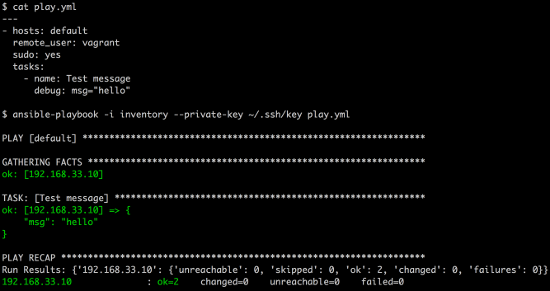
\includegraphics[scale=1.10]{play.png}
\caption{Un exemple d'exécution de playbook Ansible}
\label{}
\end{figure}

Un playbook peut contenir plusieurs \emph{plays}, qui sont un ensemble d'instructions exécutées sur un groupe de machines. Il est donc possible de configurer plusieurs types d'hosts en une seule run Ansible, contrairement à Puppet. Par exemple, au début de mon stage, l'ajout d'un noeud à l'architecture gérée par Puppet nécessitait de se logger sur le noeud, de lancer une première run puppet afin de générer une CSR (Certificate Signing Request) à l'intention de l'autorité de certification du puppetmaster, puis de se connecter sur le puppetmaster pour signer à la main cette CSR, et enfin de se reconnecter au noeud pour faire une run puppet effective. Grâce à un playbook Ansible conçu durant mon stage et contenant trois plays successives (une sur le noeud, une sur le puppetmaster et une deuxième sur le noeud), il est désormais possible d'effectuer toutes ces tâches en une seule commande ansible.

Comme pour Puppet, l'idempotence est une notion importante avec Ansible, plusieurs runs successives exécutées sur le même serveur devant retourner le même état. On peut donc être certain de l'état d'un système à l'issue d'une run vis-à-vis des configurations et des paquets installés.

\paragraph*{}Un \emph{module} Ansible est l'unité d'instruction d'Ansible. Un module est comparable à une ressource Puppet, chaque module correspondant à un script python poussé par Ansible sur les noeuds pendant une run. Il existe de nombreux modules, des plus génériques (un module \emph{raw} pour exécuter une commande ssh directe (peu recommandé)) aux plus spécifiques (par exemple \emph{rabbitmq\_plugin} pour ajouter des plugins au système de messages queue RabbitMQ)

Il est possible de rassembler un ensemble de tasks (suite d'instructions, et donc de modules), de templates, et de fichiers de variables dans une structure en arborescence appelée \emph{rôle Ansible}. On peut comparer un rôle Ansible à un module Puppet, bien que son arborescence soit un peu plus complexe, puisqu'elle ajoute des répertoires de tests, de valeurs par défaut et de handlers.

Les handlers sont des instructions appelées à l'exécution d'une instruction spéciale dans une play, l'instruction \emph{notify}. Par exemple, on peut, dans un playbook, installer un serveur web apache et pousser sa configuration à l'aide d'une template, en ajoutant l'instruction \emph{notify} lors du transfert du fichier de configuration, avec un paramètre (par exemple) "apache-reload". Si le handler du même nom est présent dans le dossier éponyme du rôle, ses instructions sont exécutées dans la foulée (dans notre cas, on reload la configuration apache juste après l'avoir modifiée)

Un rôle Ansible peut de plus être versionné sur un serveur git. Il est alors possible de l'appeler en utilisant un outil appelé ansible-galaxy, qui ira alors chercher automatiquement la dernière version du rôle. Ce système de partage des rôles permet à la fois de bénéficier de mises à jour régulières mais aussi de simplement inclure différents rôles plutôt que de réécrire un playbook à chaque fois. Par exemple, le playbook suivant installe et configure une stack Kibana + Elastic Search + Logstash uniquement en important et en exécutant des rôles Ansible :

\begin{framed}
\begin{Verbatim}[fontsize=\scriptsize]
- hosts: logs
  gather_facts: yes
  
  vars_files:
    - vars/main.yml
  pre_tasks:
    - name: Update apt cache if needed.
	  apt: update_cache=yes cache_valid_time=86400
  roles:
    - geerlingguy.java
	- geerlingguy.nginx
	- geerlingguy.elasticsearch
	- geerlingguy.elasticsearch-curator
	- geerlingguy.kibana
	- geerlingguy.logstash
	- geerlingguy.logstash-forwarder
\end{Verbatim}
\end{framed}

Cependant, au contraire de Puppet, les solutions permettant de centraliser les run et les logs Ansible à la manière d'un ensemble puppetmaster + puppetdashboard sont soit trop peu performantes, soit non Open Source et aux tarifs dissuasifs : C'est le cas notamment de la solution Ansible Tower détenue par RedHat pour centraliser une architecture d'automatisation Ansible : Le prix des licenses est suffisament élevé pour décourager l'utilisation chez Smile, et la libération des sources, si elle semble prévue par RedHat, n'a aucune date annoncée.

\subsubsection{Intégration d'Ansible à la production de Smile}

Dès mon arrivée chez Smile j'ai pu découvrir Ansible en profondeur, notamment à l'aide du très bon Ansible for DevOps\footnote{Jeff Geerling, Leanpub, 2016-11-23}, dans le but d'automatiser les processus de déploiements de plates-formes. L'une de mes premières missions chez Smile a été d'adapter un script chargé de configurer un \emph{bonding} entre deux interfaces ethernet aux dernières versions de CentOS ainsi que la configuration de bridges et de vlans. J'ai finalement migré le comportement de ce script vers Ansible, à la fois pour me permettre de mieux appréhender son fonctionnement mais aussi pour que, couplé à un déploiement d'OS en PXE, il soit possible d'automatiser entièrement le déploiement et la configuration réseau d'un nouveau serveur hôte de virtualisation. Une fois qu'a été actée la décision de passer nos nouveaux hôtes de virtualisation sous Ubuntu, ce rôle Ansible a simplement eu besoin d'être adapté pour inclure les templates de fichiers de configuration réseau de type /etc/network/interfaces.d (utilisées par Ubuntu) en plus des templates destinées aux machines sous CentOS.

J'ai ainsi pu commencer à discerner les avantages et les inconvénients d'Ansible, ainsi que ses limitations. J'ai notamment été un peu déçu par les limitations induites par le yaml, langage utilisé pour écrire les playbooks Ansible. Si plusieurs structures de contrôle sont mises en place - équivalent d'un test \emph{if} avec la ligne \emph{when} ajoutée à la fin de l'appel d'un module, possibilité d'exécuter des blocs de modules, possibilité d'appeler du code python sur les variables du playbook - le langage manque clairement de possibilités du point de vue programmation. Ce point faible fait partie intégrante de la philosophie d'Ansible : "Faire générique", s'adapter au plus grand nombre plutôt qu'aux cas particuliers. Cependant cette limitation apporte des contraintes assez lourdes, compliquant des tâches pourtant assez simples dans un shell comme par exemple effectuer l'équivalent d'un \begin{verbatim}for i in $(ls /home/fonzie); do cat $i>> /tmp/singeDuFutur.out \end{verbatim} 

En effet, pour faire une boucle sur des fichiers ou autres, il faut les lister de la manière suivante :

\begin{framed}
\begin{Verbatim}[fontsize=\scriptsize]

    # emit a debug message containing the content of each file.
    - debug:
        msg: "{{ item }}"
      with_file: # peut apparaître sous la forme "with_items"
        - first_example_file
        - second_example_file
        
\end{Verbatim}
\end{framed}

On peut donc voir que pour certaines tâches, Ansible demande des tweaks et des contorsions pour arriver à ses fins. Cependant il permet dans l'ensemble de déployer des configurations et des outils très rapidement une fois les rôles codés, ce qui a justifié le choix de l'utiliser pour déployer les hôtes de virtualisation de Smile ainsi que la base d'outils. 

L'outil \emph{ansible-galaxy} a été intégré dès le début de l'utilisation d'Ansible chez Smile, un serveur gitlab étant déjà à disposition (utilisé pour versionner les modules puppet développés par Smile). Couplé à des playbooks par défaut mis à disposition des utilisateurs, ceci permet de passer d'une durée de déploiement de nouvel host (post-PXE) d'une bonne demi-heure à quelques minutes seulement.

Pour l'instant, Ansible est utilisé pour les déploiements et les installations suivants :

\begin{itemize}
	\item La configuration réseau (bonding, vlans...)
	\item L'installation des paquets de puppet, la connexion au puppetmaster pour générer un certificat (fonctionne avec les trois puppetmasters de Smile) et la première run puppet
	\item L'installation de lxc/lxd
	\item Le déploiement de containers lxc avec quatre profils différents
\end{itemize}

\section{Upgrade de puppet}

Le chantier majeur durant mon stage chez Smile a été de mettre à jour l'infrastructure puppet, avec tous les changements de manifests et la reprise en main de l'architecture que cela implique. En effet, la précédente architecture avait été largement adaptée et modifiée par un membre de l'équipe aujourd'hui parti, sans forcément documenter tous les changements. Le passage à puppet 4 a donc été l'occasion de se réapproprier cette architecture, et de comprendre l'origine de plusieurs choix faits à cette époque (et parfois revenir sur ces choix).

\subsection{Étude de faisabilité}

Avant de migrer toute l'architecture puppet vers la version 4, j'ai commencé par rassembler des informations sur les changements introduits au passage de versions. Certains noeuds remontant jusqu'à la version 2.6, un grand nombre de fonctionnalités ont été introduits depuis, ainsi que des changements internes. Un nouveau parser de manifests a notamment été introduit, et plusieurs fonctions ont été dépréciées.

Les différences introduisant trop de \emph{breaking changes}, il a été décidé de maintenir les deux architectures en parallèle : D'une part l'existant, avec un puppetmaster jumelé en version 3 (et rétrocompatible avec les plus vieux agents puppet), d'autre part les nouvelles machines avec un puppetmaster en version 4. Pour toutes les machines de monitoring et de backup, il a donc fallu imaginer un moyen d'effectuer des runs à la fois sur puppetmaster1 (en version 3) et puppetmaster-v4, comme nous le verrons par la suite.

\subsection{Installation du serveur}

La migration vers puppet v4 avait été entamée bien avant que j'arrive chez Smile, une VM avait déjà été créée. Cependant l'équipe infra avait à l'époque eu d'autres priorités et le projet était resté à l'état embryonnaire. Une bonne partie des outils et logiciels installés étaient donc déjà remplaçables quand j'ai commencé à travailler sur la mise en place du serveur puppetmaster-v4. J'ai fait le choix de repartir sur une base vierge, en purgeant les logiciels installés avant de déployer la base du serveur puppet. L'installation en elle-même comprend :

\begin{itemize}
	\item Puppet
	\item Une base de données contenant les informations des différents noeuds, appelée puppetdb
	\item Un front-end web : puppet-dashboard, servant aussi d'ENC
	\item Nginx pour servir puppet-dashboard
\end{itemize}

Le principal problème que j'ai rencontré lors de cette installation est que le puppet-dashboard n'est plus officiellement supporté pour puppet en version 4. Il a un temps été repris par une communauté de développeurs\footnote{\url{https://github.com/sodabrew/puppet-dashboard}}, cependant le projet stagne et ne semble plus maintenu (à l'heure de rédaction de ce rapport, le dernier commit a été soumis il y a six mois). Cependant, les quelques alternatives testées ne semblaient pas adaptées : Certaines (puppetBoard, Puppet Explorer) manquent de fonctionnalités, d'autres (The Foreman) sont trop lourdes et riches en features pour l'usage de Smile, enfin certaines alternatives (Le nouveau Dashboard de puppetlabs, Puppet Enterprise Console) ne sont pas Open Source et sont donc éliminées d'office. Nous avons donc décidé de continuer à utiliser puppet-dashboard malgré la stagnation du projet. De plus, ce choix facilite la continuité et la transition entre puppet v3 et puppet v4.

\subsection{Portage des manifests puppet v3 vers puppet v4}

Une fois l'installation de puppet terminée, s'est entamée une phase durant laquelle toute l'équipe s'est mobilisée pour porter des manifests depuis puppetmaster1 vers puppetmaster-v4. Ce portage nous a permis de mieux comprendre l'architecture des manifests puppet et leur intrication dans le système de production de Smile. Comme dit plus haut, de nombreux changements et adaptations avaient été réalisés par un membre de Smile aujourd'hui parti, et cette série de portages nous a permis de réaliser à la fois la mesure de ces changements et de rationaliser leur utilité dans le nouveau système de production. La plupart du temps, ces changements ont été induits par des fonctionnalités manquant aux versions précédentes de puppet, qui ont été depuis rajoutés, comme par exemple la gestion par puppet des package repositories de Debian. Les changements de ce genre ont pu être supprimés, ce qui a conduit à purger une partie du code des manifests.

Dans d'autres cas, les comportements adoptés par les manifests n'étaient plus satisfaisants, notamment la gestion des clefs ssh des utilisateurs, dans laquelle subsistaient des reliquats de l'époque où Puppet n'était pas encore intégré à l'ingrastructure de Smile. Ces manifests ont été simplifiés et corrigés, afin d'améliorer entre autres la sécurité de l'infrastructure et sa robustesse. Par exemple, dans plusieurs cas nous avons isolé des problèmes de génération de mots de passe d'accès à des bases de données ou des daemons de backup dont la randomisation était prévisible et basée sur le hostname du noeud.

\subsection{Cas du monitoring et des backups}

Lors de la mise en place de puppetmaster-v4 un point majeur à respecter était de pouvoir conserver le monitoring et le backup des machines utilisant puppet v2/v3 tout en ajoutant la possiblité aux machines utilisant puppet v4 de déployer des configurations shinken - bacula - smile scripts v3 (un ensemble de scripts utilisé pour les backups)

Il a fallu adapter l'architecture des fichiers de puppet pour qu'il puisse s'exécuter sur deux puppetmasters sans que les changements de l'un (liste des facts, stockage des fragments de configurations...), nous avons donc déployé un clone des répertoires de travail de puppet sur chaque machine nécessitant une run puppet dédoublée. Un module puppet a été développé sur puppetmaster-v4 pour gérer spécifiquement les serveurs en run dédoublée, qui s'assure de la présence 

Les problèmes que nous avons rencontrés ensuite lors de la mise en place de ces runs dédoublées étant spécifiques à chaque technologie, je vais en parler dans deux parties différentes pour traiter les solutions apportées.

\subsubsection{Le monitoring : shinken}

Le principal problème est que puppet utilise des ressources exportées pour générer les configurations des noeuds à monitorer. En utilisant plusieurs puppetmasters, les données des noeuds ne sont donc pas stockées dans une unique puppetdb. Il a donc fallu trouver un moyen de générer les configurations en provenance des deux puppetdb sans provoquer de collision dans les configurations. En effet dans le cas de shinken, une définition d'host présente en double dans /etc/shinken/conf.d suffit à mettre en péril l'ensemble des configurations shinken, qui refuse alors de se recharger et de se rafraîchir. Ce dossier est lu récursivement par shinken au lancement du service, et tout fichier est vérifié (faute de quoi shinken reste dans l'état précédent le reload)

A l'origine, les fichiers générés par Puppet étaient stockés dans le répertoire de configuration /etc/shinken/conf.d/bypuppet, et étaient de la forme

\begin{Verbatim}[fontsize=\scriptsize]
déclaration_hostgroup{
	[...]
	déclaration du hostgroup (regroupement de plates-formes d'un même client)
	hostgroup gifi
}

déclaration host1{
	[...]
	host gifi-host1.smile-hosting.fr
}

déclaration host2{
	[...]
	host gifi-host2.smile-hosting.fr
}

déclaration host3{
	[...]
	host gifi-host3.smile-hosting.fr
}
\end{Verbatim}

A l'ajout des runs shinken sur puppet-v4, un répertoire a été ajouté pour les configurations des noeuds gérés avec puppetmaster-v4 dans /etc/shinken/conf.d/bypuppet4. Cependant avec des configurations basées sur des templates comme vue juste au-dessus, on fait face à des problèmes de double déclaration de hostgroups dans le cas où une partie des hosts d'une plate-forme sont partiellement gérés par puppetmaster1 et par puppetmaster-v4, puisque la déclaration du hostgroup est présent à la fois dans /etc/shinken/conf.d/bypuppet4 et dans /etc/shinken/conf.d/bypuppet.

Pour pallier ce problème, le module shinken a évolué à la fois sur puppetmaster1 et sur puppetmaster-v4 pour adopter un comportement permettant la coexistence des deux puppetmasters :

\begin{itemize}
	\item Les hostgroups sont maintenant définis à la fois par puppetmaster1 et puppetmaster-v4 dans /etc/shinken/conf.d/bypuppets, quitte à réécrire les mêmes fichiers dans les cas de hostgroups partagés entre les puppetmasters
	\item Les hosts sont générés dans les dossiers de leurs puppetmasters respectifs (bypuppet et bypuppet4)
\end{itemize}

Cette architecture a le mérite d'éviter les redéclarations de hostgroups, même si elle a pour inconvénient de réécrire les mêmes fichiers de configuration les uns au-dessus des autres (puppet effaçant un fichier pour réécrire, chaque run puppet v3 efface les hostgroups en commun avec puppet v4 et réciproquement)

\subsubsection{Les backups : Bacula, rsync}

\paragraph*{}Le problème posé par bacula était plus simple que celui de shinken puisque les configurations ne s'écrasaient pas d'un puppetmaster à l'autre. Il s'agissait en effet de la façon dont avait été codée une fonction ruby sensée générer des mots de passe à la volée. Cette fonction était en effet utilisée en passant en argument le fqdn du noeud puppet sur lequel elle s'exécutait, et utilisait ce fqdn comme graine pour que le même mot de passe soit généré à la fois sur le client bacula et le serveur bacula-director.

Ce comportement n'était pas souhaitable puisqu'il permet de déduire un mot de passe à l'aide d'une information très simple à obtenir.

La solution à ce problème a été de générer le mot de passe sans utiliser le fqdn comme graine, mais en exportant la ressource contenant le mot de passe. Les échanges étant sécurisés, et la puppetdb étant chiffrée, le mot de passe n'est donc plus prédictible, tout en restant partagé entre les différents noeuds.

\paragraph*{}Une partie des backups de Smile est gérée à l'aide de scripts (les Smile Scripts), basés sur rsync. Les serveurs recevant ces backups sont eux aussi en double run. Dans le cas des backups rsync, nous avons fait face à un problème de gestion des clefs ssh et des configurations du \emph{daemon} rsyncd : Les deux puppetmasters modifiant les mêmes fichiers, il a fallu adapter les manifests de manière à éviter de perdre des informations.

Pour cela, la solution apportée a été de générer les configurations et les clefs ssh des noeuds gérés par puppetmaster-v4 dans des fichiers secondaires (/etc/rsyncd.conf-v4 et /etc/ssh/authorized\_keys2). La run puppet sur puppetmaster1 cherche ensuite ces fichiers et les concatène à la fin de /etc/rsyncd.conf et /etc/ssh/root/authorized\_keys

\subsection{Mise en place des environnements de développeurs}

Une fois la base de l'infrastructure de puppetmaster-v4 installée, en même temps que le portage des manifests, des environnements ont été mis à disposition du reste de l'équipe Outsourcing de Smile afin de pouvoir travailler sur les manifests puppet et les Smile Scripts tout en ayant un versionning du code et des moyens de tester du code isolé du système de production de puppet. Pour cela il existe trois types d'environnements :
\begin{itemize}
	\item L'environnement de production, correspondant à un repository git où sont poussés uniquement les modules puppet après une phase de qualification sur un nombre restreint de serveurs
	\item L'environnement de qualification, correspondant à la branche master du repository git de développement
	\item Les environnements de développeurs, correspondant à des branches spécifiques en fonction des besoins de développement. Il est possible de faire une run puppet avec ces environnements en utilisant la commande \begin{verbatim}puppet agent --test --environment Fonzie\end{verbatim}
\end{itemize}

Il existe aussi un repository dédié au versionning des hieradata, mais celui-ci est partagé entre environnements de qualification et de production.

\subsection{Scripts de gestion de puppet}

Pour synchroniser les environnements de production et de qualification, après qu'une modification de module ait fait ses preuves sur un ensemble de serveurs de tests, nous utilisons un script ruby qui se charge d'appeler un autre script pour récapituler les différences de versions entre qualification et production, ou de rajouter les modifications de qualification vers production.

Lors du portage de ces scripts vers puppetmaster-v4, cependant, une partie des bibliothèques ruby utilisées ont été abandonnées. Ces scripts ayant été écrits par la même personne qui s'était chargée de la première version de l'infrastructure puppet, ce problème de bibliothque a été l'occasion de se réapproprier son fonctionnement, et de l'harmoniser avec les standards de Smile Outsourcing (des scripts en python et en bash)

Le script de comparaison des versions des modules puppet, basé sur le fichier metadata.json (comme vu plus haut dans la présentation de l'architecture d'un module puppet) présent dans chaque module, a donc été réécrit en bash et intégré à l'ensemble des outils Puppet.

Un autre script, qui n'était pas en place sur puppetmaster1, a été développé au cours de ce chantier. Ce script basé sur le module python \emph{pypuppetdb} permet à un utilisateur loggé sur puppetmaster-v4 de faire des appels vers la puppetdb pour accéder aux ressources (exportées ou non) d'un noeud, et permet donc de vérifier le bon fonctionnement de la génération des ressources, mais aussi de les purger dans la puppetdb, de lister les noeuds gérés par puppetmaster-v4, etc.

\chapter{Conclusion, bilan}

Au cours de mon stage, j'ai pu découvrir le monde de l'orchestration avec Puppet et Ansible, et participer à leur intégration au système de production de Smile. Aujourd'hui, la plupart des tâches d'administration et de déploiement de serveurs ne requièrent plus d'intervention directe sur un serveur, mais sont automatisées grâce à ces deux outils : Le déploiement d'un serveur "à neuf" se fait via PXE pour l'installation de l'OS, puis Ansible prend le relais pour configurer le réseau, installer puppet et les paquets essentiels. Puppet se charge de déployer les configurations de monitoring et de backup, ainsi que les configurations de bases de données, de serveurs web, d'accès ssh... Ansible permet ensuite d'installer lxc et de déployer des machines virtuelles à la volée avec des profils réseau et des accès déterminés à l'avance (VM \emph{privileged, unprivileged...})

Ces six mois m'ont beaucoup apporté puisqu'ils m'ont permis de découvrir et d'explorer le monde de l'administration système dans un système de production comptant plus d'un millier de machines, mais aussi le monde de l'entreprise (ce que mes deux stages précédents, l'un en recherche, l'autre dans une entreprise d'une seule personne, ne m'avaient pas permis d'appréhender) et du service. J'ai également beaucoup appris sur les concepts liés à l'automatisation et à l'orchestration, qui, je pense, est un sujet qui va devenir de plus en plus présent dans le milieu de l'administration système dans les prochaines années.

Ce stage a donc parfaitement répondu à mes attentes puisque je souhaitais effectuer un stage orienté technique et touchant de nombreux champs d'application, afin de pouvoir explorer un maximum d'aspects des métiers de l'administration système, tout en n'étant pas enfermé dans un seul système comme ç'aurait pu être le cas en travaillant sur un système interne à une entreprise. L'aspect Open Source de ce stage me semblait également intéressant, tant par conviction personnelle que pour confirmer qu'il est possible de construire de belles choses, des infrastructures robustes et efficaces, sans pour autant se limiter à des outils opaques.

Enfin, avec Smile j'ai pu découvrir une équipe dynamique et agréable, construite autour d'une même conception de l'informatique et d'un amour pour l'Open Source ; Équipe avec laquelle j'aurai le plaisir de continuer à travailler une fois ce stage terminé.

\appendix
\chapter{Exemple de code puppet}

Je vais maintenant présenter un module puppet typique, chargé de mettre en place les configurations pour faire des backups bacula.

Le module a la structure suivante :

\begin{Verbatim}[fontsize=\scriptsize]
magui@puppetmaster-v4:~/puppet/modules/bacula (master)$ tree
.
+-- files
|   \-- init-bacula.conf
+-- manifests
|   +-- client
|   |   +-- config.pp
|   |   +-- package.pp
|   |   \-- service.pp
|   +-- client.pp
|   +-- director
|   |   \-- nrpe.pp
|   +-- director.pp
|   +-- storage
|   |   +-- config.pp
|   |   +-- package.pp
|   |   \-- service.pp
|   \-- storage.pp
+-- metadata.json
\-- templates
    +-- backuptracker.d
    |   \-- hostname.bacula.erb
    +-- bacula-sd.conf.erb
    +-- node-bacula-dir.conf.erb
    +-- node-bacula-fd.conf.erb
    \-- node-bacula-sd.conf.erb
\end{Verbatim}

Nous ne présenterons qu'une partie de ce module, la partie chargée de générer la configuration des clients bacula (le fichier client.pp et le contenu du répertoire client)

Tout d'abord, présentons le fichier client.pp

\begin{framed}
\begin{Verbatim}[fontsize=\scriptsize]
# Bacula client class: applies to each node which is saved using Bacula.
# Each client needs 3 files (sd,fd,dir) sharing 2 different passwords :
# - between SD and DIR
# - between FD and DIR
# Passwords are randomly generated in a way which is replayable: (we can
# "randomly" regenerate the same passwords given the FQDN and the CA RSA key.pem
# file.
#
class bacula::client {
  if $racktables_platform_code == undef or $racktables_platform_code == 'unknown' {
    warning("Unable to determine $fqdn's platform_code. Check Racktables.")
  }
  else {
    puppetnode::announce::register { $title: }
    include bacula::client::package
    include bacula::client::config
    include bacula::client::service
  }
}\end{Verbatim}
\end{framed}

Ce fichier, contenu à la racine du dossier \emph{manifests}, vérifie tout d'abord que la hiera (l'équivalent d'une variable) \$racktables\_platform\_code est bien définie. Suite à quoi, elle instancie une classe puppetnode::announce::register avec en argument la hiera \$title ; Cette classe permet d'informer les utilisateurs d'un serveur des classes puppet utilisées sur ce serveur en ajoutant une ligne au \emph{motd} (message of the day) affiché lors de la connexion.

Après cette action, elle inclut trois fichiers inclus dans le dossier client : package.pp, config.pp et service.pp

\subsubsection*{package.pp}

Commençons par examiner package.pp :

\begin{framed}
\begin{Verbatim}[fontsize=\scriptsize]
# install bacula file-daemon package
class bacula::client::package {
  $bacula_fd = hiera_hash("bacula-fd")
  package { $bacula_fd['package']:
    ensure  => present,
  }
}\end{Verbatim}
\end{framed}

Le fichier package.pp est généralement utilisé pour installer les paquets nécessaires au fonctionnement d'un système. La notation \$bacula\_fd = hiera\_hash("bacula-fd") permet de stocker dans la variable puppet \$bacula\_fd non pas une valeur unique, mais une table de hachage (tableau de paires clés/valeurs) stockée sous forme de hieradata.

L'exécution de la ressource \emph{package} sur cette table de hachage permet d'installer l'ensemble des paquets listés dedans. En changeant la ligne
\begin{Verbatim}[fontsize=\scriptsize]
    ensure  => present,
\end{Verbatim}

par la ligne

\begin{Verbatim}[fontsize=\scriptsize]
    ensure  => absent,
\end{Verbatim}
on peut à la place désinstaller les paquets listés dans la hiera.

Dans le cas du client bacula, le seul paquet installé par puppet est le paquet \emph{bacula-client}

\subsubsection*{service.pp}

Le contenu du fichier service.pp :

\begin{framed}
\begin{Verbatim}[fontsize=\scriptsize]
# Ensure bacula-fd will start
class bacula::client::service {
  require bacula::client::package
  require bacula::client::config
  $bacula_fd = hiera_hash("bacula-fd")

  service { $bacula_fd['service']:
    ensure  => running,
    enable  => true,
  }
}\end{Verbatim}
\end{framed}

La ressource \emph{service} permet de lancer (enable => true), d'arrêter ou de redémarrer des services system V ou des units systemd.

La particularité de ce fichier est qu'il contient deux conditions d'ordonnancement \emph{require}, qui sont donc appliquées avant le contenu de la classe service elle-même.

\subsubsection*{config.pp}

Le fichier le plus important est config.pp : 

\begin{framed}
\begin{Verbatim}[fontsize=\tiny,numbers=left]
class bacula::client::config {
  require bacula::client::package

  $bacula_fd = hiera_hash("bacula-fd")
  validate_hash( $bacula_fd )

  # Required by the template
  $piddir = $bacula_fd['piddir']
  $datadir = $bacula_fd['datadir']
  validate_absolute_path( $piddir, $datadir)

  # Per-node storage daemon configuration:
  $bacula_sd_config = hiera_hash('bacula-sd-config', undef)
  if $bacula_sd_config != undef {
    validate_hash( $bacula_sd_config )
    $bacula_sd_address = $bacula_sd_config['address']
    $bacula_sd_device = chompchar($bacula_sd_config['device'], "/")
    validate_absolute_path( $bacula_sd_device )
    validate_string( $bacula_sd_address )

    # Global storage daemon configuration (available storages and devices)
    $bacula_sd_data = hiera_hash('bacula-sd-data')

    $valid_sd_addresses = keys($bacula_sd_data)
    validate_array( $valid_sd_addresses )
    if !($bacula_sd_address in $valid_sd_addresses ) {
      $valid_sd_addresses_str = join( $valid_sd_addresses, ',')
      fail("Invalid storage daemon device $bacula_sd_device. Valids are '$target_sd_devices_str'")
    }

    $valid_sd_devices = $bacula_sd_data[$bacula_sd_address]['devices']
    # If the storage device given is incorrect: print an error and fail the compilation
    if !($bacula_sd_device in $valid_sd_devices) {
      $target_sd_devices_str = join( $valid_sd_devices, ',')
      fail("Invalid storage daemon device $bacula_sd_device. Valids are '$target_sd_devices_str'")
    }

	$bacula_pwd = genpasswd(45, $hostname)
    $bacula_dir_config = hiera_hash('bacula-director-config')
    $bacula_dir_address = $bacula_dir_config['address']
    $bacula_full_retention = 61# $bacula_dir_config['full-retention'].scanf("%i")
    $bacula_full_interval = $bacula_dir_config['full-interval']
    $bacula_diff_retention = $bacula_dir_config['diff-retention']
    $bacula_job_retention = $bacula_dir_config['job-retention']
    $bacula_job_definition = $bacula_dir_config['job-definition']

    validate_string($bacula_dir_address)
    if $bacula_dir_address == undef {
      fail("Variable bacula_dir_address is undef.")
    }

    file { $bacula_fd['cfgfile']:
      ensure  => present,
      content => template("bacula/node-bacula-fd.conf.erb"),
      notify  => Service[$bacula_fd['service']],
    }

    $bacula_dir_mv_cmd = "bacula-dir-config-mv-${hostname}-conf-to-old"

    ## Export config file on 'targeted' bacula director
    @@file { "$bacula_dir_cfgdir/${hostname}.conf":
      ensure  => present,
      content => template("bacula/node-bacula-dir.conf.erb"),
      notify  => Exec[$bacula_dir_mv_cmd],
      tag     => [$environment, $bacula_dir_address, "per-node-config-bacula-dir"],
    }

    # When exporting, move the old config file in a safe place
    @@exec { $bacula_dir_mv_cmd:
      refreshonly => true,
      path        => ['/usr/bin', '/usr/sbin', '/bin'],
      command     => "mv /etc/bacula/config/${hostname}.conf /etc/bacula/config-old/${hostname}.conf",
      onlyif      => "test -f /etc/bacula/config/${hostname}.conf",
      tag         => [$environment, $bacula_dir_address, "per-node-config-bacula-dir"],
    }

    # This command will create a new catalog if it does not exists
    @@exec { "bacula-dir-create-catalog-${hostname}":
      path        => ['/usr/bin', '/usr/sbin', '/bin'],
      command     => "/etc/bacula/smile-scripts/create_catalog.sh ${hostname}",
      unless      => "sudo -u postgres psql -c '\\l' | grep '${hostname}-catalog'",
      tag         => [$environment, $bacula_dir_address, "per-node-config-bacula-dir"],
    }

    $bacula_sd_mv_cmd = "bacula-sd-config-mv-${hostname}-conf-to-old"

    ## Export config file on 'targeted' bacula storage daemon
    @@file { "$bacula_sd_cfgdir/${hostname}.conf":
      ensure  => present,
      content => template("bacula/node-bacula-sd.conf.erb"),
      notify  => [ Exec[$bacula_sd_mv_cmd], Service[$bacula_sd['service']] ],
      tag     => [$environment, $bacula_sd_address, "per-node-config-bacula-sd"],
    }

    # When exporting, move the old config file in a safe place
    @@exec { $bacula_sd_mv_cmd:
      path        => ['/usr/bin', '/usr/sbin', '/bin'],
      refreshonly => true,
      command     => "mv /etc/bacula/config/${hostname}.conf /etc/bacula/config-old/${hostname}.conf",
      onlyif      => "test -f /etc/bacula/config/${hostname}.conf",
      tag         => [$environment, $bacula_sd_address, "per-node-config-bacula-sd"],
    }
    file { $datadir:
      ensure  => directory,
      owner   => 'bacula',
      group   => 'bacula',
    }

    file { $piddir:
      ensure  => directory,
      owner   => 'bacula',
      group   => 'daemon',
    }
  }
  else {
    fail("No bacula configuration done because hiera 'bacula-sd-config' key not found.")
  }
}\end{Verbatim}
\end{framed}

Pour le résumer, ce code génère un mot de passe aléatoire, le stocke dans la puppetdb (le préfixe @@ devant une ressource permet de l'exporter) et exporte plusieurs fichiers de configurations basés sur des templates (localisées dans /bacula/templates/). On peut voir deux types de ressources principales : Les ressources de type \emph{exec} permettent d'exécuter une commande directement sur un noeud (par exemple mv /etc/bacula/config/${hostname}.conf /etc/bacula/config-old/${hostname}.conf), et les ressources de type \emph{file} qui permettent de pousser un fichier, soit en copiant un fichier depuis une URL, soit en remplissant une template.

\chapter{Exemple de code Ansible}
\end{document}
